\documentclass[11pt,a4paper]{article}
\usepackage[T1]{fontenc}
\usepackage[utf8]{inputenc}
\usepackage{lmodern}
\usepackage[margin=2.5cm]{geometry}
\usepackage{amsmath,amssymb}
\usepackage{booktabs}
\usepackage{graphicx}
\usepackage{verbatim}
\usepackage{microtype}
\usepackage[hidelinks]{hyperref}

% generado por datos_nota.py -- no editar a mano
\newcommand{\semillasCasa}{65{,}535}
\newcommand{\gensCasa}{100}
\newcommand{\extintasCasa}{15{,}335}
\newcommand{\sincerrarCasa}{11{,}760}
\newcommand{\evaluadasCasaSemillas}{51{,}472}
\newcommand{\trasladadasCasa}{14{,}063}
\newcommand{\sincerrarpctCasa}{22.8}
\newcommand{\asentadasCasa}{24{,}377}
\newcommand{\sopadensCasa}{0.122}
\newcommand{\sopasCasa}{40}
\newcommand{\sopaladoCasa}{128}
\newcommand{\sopagensCasa}{600}
\newcommand{\sopainicialCasa}{0.30}
\newcommand{\semillasConway}{65{,}535}
\newcommand{\gensConway}{100}
\newcommand{\extintasConway}{15{,}492}
\newcommand{\sincerrarConway}{9{,}284}
\newcommand{\evaluadasConwaySemillas}{51{,}472}
\newcommand{\trasladadasConway}{14{,}063}
\newcommand{\sincerrarpctConway}{18.0}
\newcommand{\asentadasConway}{26{,}696}
\newcommand{\sopadensConway}{0.052}
\newcommand{\sopasConway}{40}
\newcommand{\sopaladoConway}{128}
\newcommand{\sopagensConway}{600}
\newcommand{\sopainicialConway}{0.30}
\newcommand{\objetosCasa}{96}
\newcommand{\objetosConway}{81}
\newcommand{\pobDiez}{11}
\newcommand{\minDiez}{B37/S238}
\newcommand{\maxDiez}{B378/S2378}
\newcommand{\semillasDiez}{8}
\newcommand{\pobTreintaydos}{13}
\newcommand{\minTreintaydos}{B37/S237}
\newcommand{\maxTreintaydos}{B378/S2378}
\newcommand{\semillasTreintaydos}{8}
\newcommand{\evaluadasCasa}{471}
\newcommand{\muestraCasa}{25}
\newcommand{\lejosCasa}{1{,}000}
\newcommand{\crecCasaAcotada}{71}
\newcommand{\crecCasaCrece}{338}
\newcommand{\crecCasaCierra}{62}
\newcommand{\lejoslejosCasa}{5{,}000}
\newcommand{\lejosnCasa}{10}
\newcommand{\evaluadasConway}{465}
\newcommand{\muestraConway}{20}
\newcommand{\lejosConway}{1{,}500}
\newcommand{\crecConwayCierra}{191}
\newcommand{\crecConwayAcotada}{268}
\newcommand{\crecConwayCrece}{6}
\newcommand{\lejoslejosConway}{20{,}000}
\newcommand{\lejosnConway}{6}
\newcommand{\lejosCreceCasa}{8}
\newcommand{\lejosRecurreConway}{6}
\newcommand{\recurremaxConway}{4{,}100}
\newcommand{\recurreminConway}{1{,}700}
\newcommand{\ajustedesde}{1{,}000}
\newcommand{\expmin}{1.73}
\newcommand{\expmax}{2.12}
\newcommand{\expmed}{1.85}
\newcommand{\expn}{8}
\newcommand{\velmin}{0.056}
\newcommand{\velmax}{0.065}
\newcommand{\densmin}{0.111}
\newcommand{\densmax}{0.130}
\newcommand{\frentelado}{1{,}600}
\newcommand{\frentegens}{2{,}400}
\newcommand{\frentebloque}{16}
\newcommand{\frenteumbral}{0.03}

% The only number not taken from data/: the apgsearch trial of the section on
% Catagolue, measured by hand on the apgsearch build (not part of this package).
\newcommand{\apgsopas}{1{,}000}

\title{The Life-like rule B37/S2378:\\
an exhaustive census of $4\times4$ seeds, disk-shaped growth,\\
and two oscillators with machine-checked periods}
\author{Joel Cruz Cabrera\thanks{ORCID \href{https://orcid.org/0009-0005-4048-1237}{0009-0005-4048-1237}.}}
\date{September 2026 (v2)}

\begin{document}
\maketitle

\begin{abstract}
The outer-totalistic rule B37/S2378 (a dead cell is born with 3 or 7 live neighbours;
a live cell survives with 2, 3, 7 or 8) is a close relative of DryLife (B37/S23).
We report the first census of it that we could find. Every one of the
\evaluadasCasaSemillas{} seeds whose bounding box is exactly $4\times4$ was evolved until it
recurred up to translation; the same protocol was run for Conway's B3/S23 as a control. The
B37/S2378 census yields \objetosCasa{} objects, including an oscillator of period~10
(\pobDiez{} cells) and one of period~32 (\pobTreintaydos{} cells), neither of which
exists under B3/S23. Seeds that do not settle behave very differently in the two rules:
under B37/S2378, \crecCasaCrece{} of \evaluadasCasa{} sampled unsettled seeds are
still growing after \lejosCasa{} generations, as a disk whose interior holds the density
of random soup (\densmin--\densmax) and whose edge advances at
\velmin--\velmax{}\,$c$; under B3/S23 none of the \evaluadasConway{} sampled
unsettled seeds keeps growing (the \crecConwayCrece{} still growing at \lejosConway{}
generations all settle by \lejoslejosConway). The periods of both oscillators,
the minimality of the period~10, and the failure of the period-10 pattern under
Conway's rule are proved in Lean~4 by kernel computation, with no axioms beyond the
standard ones.
\end{abstract}

\section{The rule}

A Life-like rule is written B$x$/S$y$: a dead cell with $n$ live Moore neighbours
becomes live if $n\in x$, and a live cell stays live if $n\in y$. Conway's Game of Life
is B3/S23~\cite{gardner1970}. The rule studied here adds birth on 7 and survival on 7
and 8. Its nearest named relative is DryLife, B37/S23, whose explosive behaviour is
known in the community~\cite{lifewiki-lifelike}; survival on 7 and 8 lets crowded
regions persist instead of thinning out. Eppstein~\cite{eppstein} discusses which
Life-like rules can support both growth and decay.

\section{Method}

\paragraph{Exhaustive census.} Of the $2^{16}-1=\semillasCasa$ non-empty patterns of a
$4\times4$ box, the \trasladadasCasa{} that do not touch all four sides are translates of
patterns of a smaller box and are left out; each of the remaining
\evaluadasCasaSemillas{}, whose bounding box is exactly $4\times4$, is evolved alone in the
plane (on a board with
a margin larger than the number of generations, so the boundary is never reached) for
up to \gensCasa{} generations. The whole pattern is compared, after cropping, with
every earlier generation; the first exact repetition up to translation fixes the
outcome: a still life (period 1, no shift), an oscillator (period $p>1$, no shift) or a
spaceship (a shift). A seed that dies is \emph{extinct}; a seed that has not repeated
by the last generation is \emph{unsettled}. The settled final pattern is split into
objects: live cells at Chebyshev distance at most~3 belong to the same object, so
objects close enough to interact are counted together. Objects are identified up to the
eight symmetries of the square and, for oscillators and spaceships, across all their
phases.

\paragraph{Soups.} \sopasCasa{} random soups of side \sopaladoCasa{} on a torus, initial
density \sopainicialCasa, evolved for \sopagensCasa{} generations; we record the
live-cell density.

\paragraph{Growth of unsettled seeds.} One unsettled seed in every \muestraCasa{}
(B37/S2378) or every \muestraConway{} (B3/S23) is evolved further, to \lejosCasa{} and
\lejosConway{} generations respectively, and classified as growing (population still
rising in the last window), bounded, or settling. A subsample of the growing seeds is
followed further still (\lejoslejosCasa{} and \lejoslejosConway{} generations),
removing escaping gliders once they are more than 20 cells from the core so that they
do not inflate the bounding box.

\paragraph{The front.} Three growing seeds are evolved for \frentegens{} generations
on a \frentelado{}$\times$\frentelado{} board. The board is divided into
$\frentebloque\times\frentebloque$ blocks; the \emph{core} is the set of blocks with
density above \frenteumbral{} (a lone glider in a block has density $5/256<0.02$),
its radius is $\sqrt{\text{area}/\pi}$ and its density is the mean over its blocks.

\section{Results}

\subsection{The census}

Table~\ref{tab:censo} compares the two rules. Of the \evaluadasCasaSemillas{} seeds,
\extintasCasa{} die out and \sincerrarCasa{} (\sincerrarpctCasa\,\%) are unsettled
under B37/S2378, against \extintasConway{} and \sincerrarConway{}
(\sincerrarpctConway\,\%) under B3/S23. The only spaceship reached from a $4\times4$
seed is, in both rules, the glider, which B37/S2378 inherits unchanged. The two
columns differ in the oscillators: B37/S2378 has one of period~10 and one of
period~32, each reached from \semillasDiez{} seeds, and neither occurs under B3/S23.

\begin{table}[h]
\centering
% generado por datos_nota.py -- no editar a mano
\begin{tabular}{lrrrr}
\toprule
 & \multicolumn{2}{c}{B37/S2378} & \multicolumn{2}{c}{B3/S23} \\
\cmidrule(lr){2-3}\cmidrule(lr){4-5}
class & objects & occurrences & objects & occurrences \\
\midrule
still life & 66 & 27{,}917 & 55 & 22{,}676 \\
oscillator, $p=2$ & 26 & 9{,}000 & 24 & 7{,}972 \\
oscillator, $p=3$ & 1 & 24 & 1 & 48 \\
oscillator, $p=10$ & 1 & 8 & -- & -- \\
oscillator, $p=32$ & 1 & 8 & -- & -- \\
spaceship, $p=4$ (glider) & 1 & 752 & 1 & 728 \\
\midrule
total & 96 & 37{,}709 & 81 & 31{,}424 \\
\bottomrule
\end{tabular}

\caption{Objects reached from the \evaluadasCasaSemillas{} seeds whose bounding box is
exactly $4\times4$. \emph{Objects} counts distinct objects up to symmetry and phase;
\emph{occurrences} counts how many times each appears in the final patterns (a seed
can end in several objects). Cells within Chebyshev distance 3 belong to the same object.}
\label{tab:censo}
\end{table}

\subsection{Two oscillators}

Figure~\ref{fig:osc} shows one phase of each oscillator; their RLE follows.
\verbatiminput{p10.rle}
\verbatiminput{p32.rle}

\begin{figure}[h]
\centering
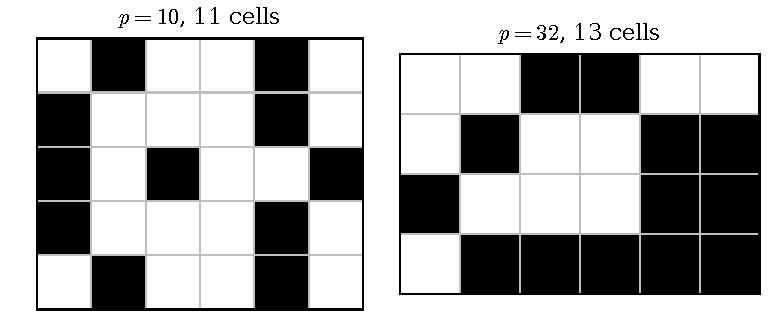
\includegraphics[width=0.75\textwidth]{fig_osciladores.pdf}
\caption{One phase of the period-10 and period-32 oscillators of B37/S2378.}
\label{fig:osc}
\end{figure}

\paragraph{Rule range.} An oscillator works in every rule that agrees with B37/S2378
on the neighbour counts that actually occur during its cycle. Recording, over one
period, which counts cause a birth or a survival and which counts occur without one
gives the range. The period-10 oscillator works exactly in the rules from
\minDiez{} to \maxDiez{}, and the period-32 one from \minTreintaydos{} to
\maxTreintaydos{}. Both need birth on 7, so neither can exist in Conway's rule or in any
rule without B7.

\paragraph{Prior occurrence.} As of 26 September 2026, Catagolue~\cite{catagolue} has
no census for any of the six rules in these two ranges, LifeWiki's lists of Life-like
rules~\cite{lifewiki-lifelike,lifewiki-universal} do not list B37/S2378, and a code
search of public GitHub repositories finds no pattern file for any of the six rule
strings. We found no earlier description of these two oscillators; we could not
search the ConwayLife forum, and a claim of novelty should be read with that in mind.

\paragraph{Machine-checked periods.} The oscillators are encoded in Lean~4~\cite{lean4} on a finite
board wide enough that no live cell ever reaches its border during the cycle (margins
of 4 and 7 cells), so the finite evolution coincides with the evolution in the plane.
The following are proved by \texttt{decide}, i.e.\ by evaluation in the kernel, without
\texttt{native\_decide}:
\begin{itemize}
\item \texttt{p10\_period}: 10 steps of B37/S2378 return the period-10 pattern to itself;
\item \texttt{p10\_period\_minimal}: no smaller number of steps does;
\item \texttt{p32\_period}: 32 steps return the period-32 pattern to itself;
\item \texttt{p10\_not\_conway}: under B3/S23 the period-10 pattern does not return to
itself within 10 steps.
\end{itemize}
\texttt{\#print axioms} reports only \texttt{propext}. The development builds with
Lean~v4.33.0 and a pinned Mathlib~\cite{mathlib} and accompanies this note. The border condition is
checked by our simulation, not by Lean, and the minimality of the period~32 is also
computational (the census finds no earlier repetition).

\subsection{Random soups}

Random soups settle to a density of \sopadensCasa{} under B37/S2378, against
\sopadensConway{} under B3/S23 (Figure~\ref{fig:sopa}). The larger value is what one
expects from survival on 7 and 8: dense clusters that B3/S23 would erode persist.

\begin{figure}[h]
\centering
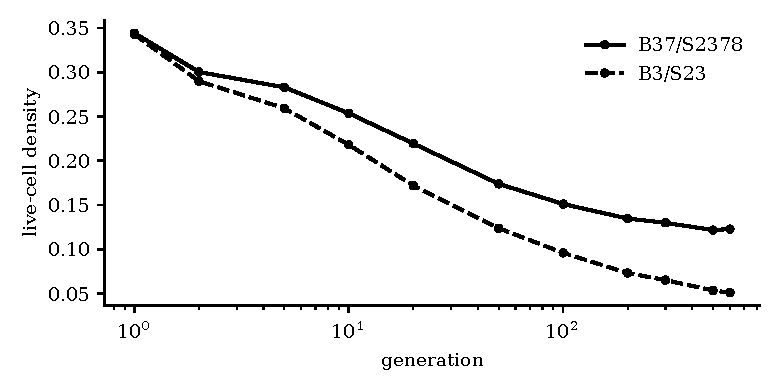
\includegraphics[width=0.75\textwidth]{fig_sopa.pdf}
\caption{Live-cell density of random soups (mean of \sopasCasa{} soups of side
\sopaladoCasa, torus, initial density \sopainicialCasa).}
\label{fig:sopa}
\end{figure}

\subsection{Unbounded growth}

Of the \evaluadasCasa{} sampled unsettled seeds of B37/S2378, \crecCasaCrece{} are
still growing after \lejosCasa{} generations, \crecCasaAcotada{} are bounded but
unsettled and \crecCasaCierra{} settle. Of the \evaluadasConway{} sampled unsettled
seeds of B3/S23, \crecConwayCrece{} are still growing after \lejosConway{}
generations; followed to \lejoslejosConway{} generations, all \lejosRecurreConway{}
settle, between generation \recurreminConway{} and \recurremaxConway{}. Under
B37/S2378, \lejosCreceCasa{} of the \lejosnCasa{} seeds followed to \lejoslejosCasa{}
generations are still growing; fitting population $\propto t^{\alpha}$ between
generations \ajustedesde{} and \lejoslejosCasa{} gives $\alpha$ between \expmin{} and \expmax{} (median
\expmed, $n=\expn$).

The growth is a disk. For the three seeds of Figure~\ref{fig:frente} the core radius
grows linearly, with speeds between \velmin{} and \velmax{} cells per generation, and
the density inside the core stays between \densmin{} and \densmax{}, the density that
random soup settles to. The picture is therefore a region of settled-soup texture whose
edge keeps converting empty space at a roughly constant speed, which makes the area,
and so the population, quadratic in time; the fitted exponents below 2 reflect the
early, not yet circular, stage. Gliders escape from the edge throughout.

\begin{figure}[h]
\centering
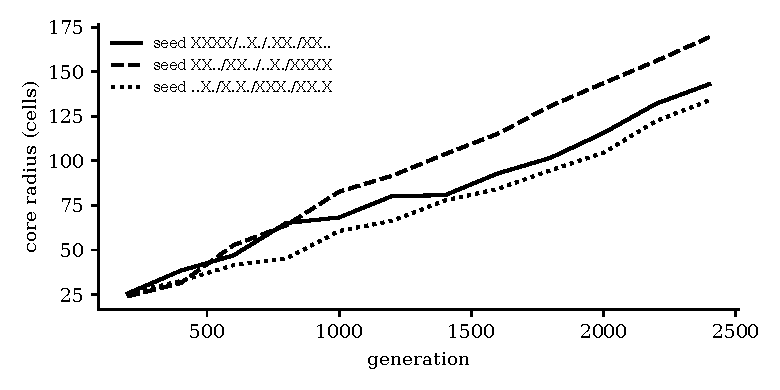
\includegraphics[width=0.75\textwidth]{fig_frente.pdf}
\caption{Core radius of three growing $4\times4$ seeds of B37/S2378 (blocks of
$\frentebloque\times\frentebloque$ cells with density above \frenteumbral).}
\label{fig:frente}
\end{figure}

\subsection{Why there is no Catagolue census}

Catagolue's search program, apgsearch~\cite{catagolue}, runs each soup until it
stabilises, with a budget of the order of $10^5$ generations. Under B37/S2378 a
typical soup does not stabilise: it grows as the disk above, so the work per generation
grows with the square of the generation count. In our trial, a build of apgsearch configured
for B37/S2378 had not completed \apgsopas{} soups after nine minutes, where B3/S23 takes a
fraction of a second. The rule is uncensused because the census method assumes soups
that settle, not because it was overlooked.

\section{Limitations}

The census covers only the $4\times4$ box and only objects reached from it. The growth
statistics come from samples (one seed in \muestraCasa{} and one in \muestraConway),
and the front was measured on three seeds. The rule-range statement and the border
condition for the Lean encoding are established by computation, not by proof. The
novelty statement rests on the sources listed above.

\section*{Data and code}

The census, soup, growth and front scripts, their JSON outputs, the script that
generates every number, table and figure in this note from those outputs, the RLE
files and the Lean development are deposited with this note and kept, with unit tests
and continuous integration that rebuilds the Lean proofs and audits their axioms, at
\url{https://github.com/joelcanary/life-like-rule-b37s2378}. Every number in the text
is produced by that script; none is typed by hand.

\section*{Version history}

\textbf{v2} (26 September 2026). Corrects the number of seeds the census evolves: the
\evaluadasCasaSemillas{} whose bounding box is exactly $4\times4$, not all
\semillasCasa{} non-empty patterns of the box as v1 stated, and the percentages derived
from it. Adds the citations of Lean~4 and Mathlib and the link to the code repository.
No other result changes.

\section*{Use of AI assistance}

The computations, scripts and a first draft of this text were prepared with the help
of an AI assistant (Claude, Anthropic). The author reviewed the results and is
responsible for the content.

\begin{thebibliography}{9}
\bibitem{gardner1970}
M.~Gardner, \emph{Mathematical Games: The fantastic combinations of John Conway's new
solitaire game ``life''}, Scientific American 223 (1970), 120--123.
\bibitem{lifewiki-lifelike}
LifeWiki, \emph{List of Life-like rules},
\url{https://conwaylife.com/wiki/List_of_Life-like_rules} (accessed 26 September 2026).
\bibitem{lifewiki-universal}
LifeWiki, \emph{List of universal cellular automata},
\url{https://conwaylife.com/wiki/List_of_universal_cellular_automata} (accessed
26 September 2026).
\bibitem{catagolue}
A.~P.~Goucher, \emph{Catagolue} and \emph{apgsearch},
\url{https://catagolue.hatsya.com} (accessed 26 September 2026).
\bibitem{eppstein}
D.~Eppstein, \emph{Growth and decay in Life-like cellular automata}, in A.~Adamatzky
(ed.), \emph{Game of Life Cellular Automata}, Springer (2010), 71--97;
arXiv:0911.2890.
\bibitem{lean4}
L.~de~Moura and S.~Ullrich, \emph{The Lean~4 theorem prover and programming language},
in \emph{Automated Deduction -- CADE 28}, LNCS 12699, Springer (2021), 625--635.
\bibitem{mathlib}
The mathlib Community, \emph{The Lean mathematical library}, in \emph{Proceedings of
the 9th ACM SIGPLAN International Conference on Certified Programs and Proofs (CPP
2020)}, ACM (2020), 367--381.
\end{thebibliography}

\end{document}
